\chapter{Algorithmen zur Pfadplanung}\index{Algorithmen}\index{Pfadplanung}\index{Algorithmus}
In diesem Kapitel werden die Algorithmen \emph{Dijkstra} und \emph{Bellman-Ford} zur Pfadplanung beschrieben.

\section{Einleitung}
\label{Was ist Pfadplanung?}
Die Pfadplanung ist ein nichtdeterministisches Problem mit polynomialer Laufzeit ("NP"), bei dem es darum geht, einen Pfad zu finden, 
der in einem System den Ausgangspunkt mit dem Ziel verbindet. Der zu wählende Weg (die beste Route) wird durch Beschränkungen 
und Bedingungen bestimmt \cite{Karur:21}.

In der Informatik, insbesondere in der Graphentheorie, ist das Problem des kürzesten Weges bekannt. Der kürzestmögliche Weg von 
einer Quelle zu einem Ziel hat die geringsten Längenanforderung.

Die Dijkstra- und Bellman-Algorithmen für den kürzesten Weg sind in einer Vielzahl von Bereichen und Anwendungen
weit verbreitet. Beispiele für diese Anwendungen sind Routing-Protokolle für Netzwerke, Routenplanung, 
Verkehrssteuerung, Pfadfindung in sozialen Netzwerken, Computerspiele und Navigationssysteme \cite{Panda:18}.

\section{Uninformierte Suche}
\label{Uninformierte Suche}
Als Einstieg in die Thematik der Pfadplanung wird die Uninformierte Suche beschrieben.
Uninformierte Algorithmen werden auch „blind“ genannt, weil bei ihrer 
Suche auf keine zusätzlichen Informationen (wie z.B. Gewichtungen) zurückgegriffen wird \cite[80-82]{Russell:10}.

Nach \cite[80-82]{Russell:10} gibt es 4 Hauptkriterien nach denen Pfachsuchalgorithmen bewertet werden können:
\begin{itemize}
	\item \emph{Vollständigkeit}: Liefert der Algorithmus immer eine Lösung, wenn es eine Lösung gibt?
	\item \emph{Optimalität}: Liefert der Algorithmus einen optimalen Weg?
	\item \emph{Zeitkomplexität}: Wie lange dauert es bis der Algorithmus einen Weg gefunden hat?
	\item \emph{Raumkomplexität}: Wie viel Speicher wird benötigt um die Lösung zu finden?
\end{itemize}
\newpage
\subsection{Breitensuche}
\label{Breitensuche}
Die Breitensuche gehört zu den uninformierten Suchalgorithmen. 
Der erste Schritt der Breitensuche ist es, wie man in Abb \ref{fig:Breitensuche} sehen kann, alle verbundenen Knoten ersten Grades des Wurzelknotens zu besuchen \cite[80-82]{Russell:10}.
Erst dann wird die nächste Ebene besucht. Dies wird Ebene für Ebene im Baum wiederholt, bis alle Knoten besucht wurden. 
Die Breitensuche ist vollständig und bei z.B gleichverteilten Aktionskosten auch optimal \cite[80-82]{Russell:10}.
\begin{figure}
	\centering
	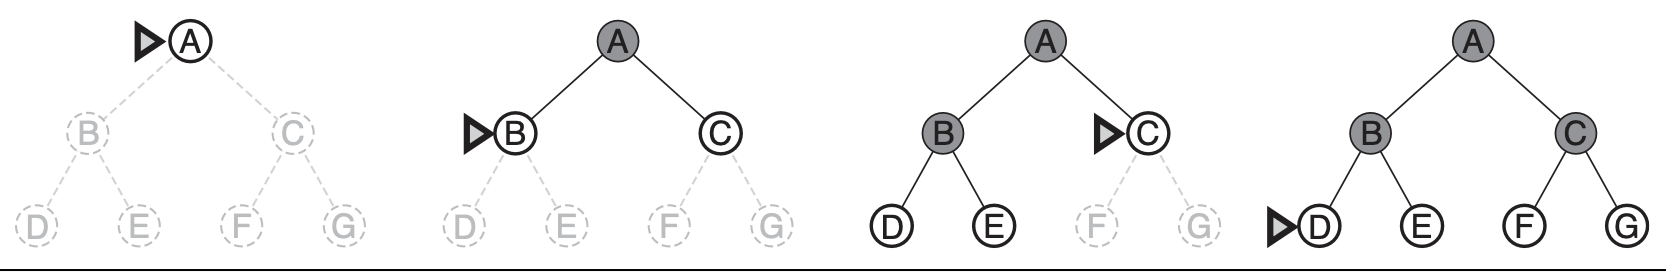
\includegraphics[width=1.0\textwidth]{images/breitensuche.png}
	\caption{Breitensuche in einem Binärbaum. Unbesuchte Knoten werden hellgrau dargestellt, besuchte Knoten werden dunkelgrau dargestellt.}
	\label{fig:Breitensuche}
\end{figure}
\\
\newpage
\subsection{Tiefensuche}
\label{Tiefensuche}
Die Tiefensuche gehört ebenfalls zu den uninformierten Suchalgorithmen.
Das Vorgehen bei der Tiefensuche ist es, wie man in Abb. \ref{fig:Tiefensuche} sehen kann, zuerst alle Unterknoten eines direkten Nachbarn (z.B Knoten $B$) des Wurzelknotens $A$ zu besuchen bis dieser 
keine unbesuchten Unterknoten mehr hat \cite[85,86]{Russell:10}.
Erst dann wird der nächste Nachbar, in Abb. \ref{fig:Tiefensuche} Knoten $C$, in der ersten Ebene besucht, bis keine unbesuchten Knoten mehr vorhanden sind oder der Zielknoten gefunden wurde \cite[85,86]{Russell:10}.
Es gibt 2 Versionen der Tiefensuche: die Version, die in einem Graphen einen kürzesten Weg zu einem Ziel sucht, und die Version, 
die in einer Baumstruktur den kürzesten Weg sucht \cite[85,86]{Russell:10}.
Nur die Version, welche in einem Graphen sucht, ist in endlicher Raumkomplexität vollständig, die Version mit Baumstruktur ist leider nicht vollständig. \cite[85,86]{Russell:10}.

Die Tiefensuche ist (indirekt) an vielen komplexeren Algorithmen beteiligt. 
So führt die iterative Vertiefungssuche die klassische Tiefensuche wiederholt und in Verbindung mit einer steigenden 
Tiefenbegrenzung aus, bis ein Ziel gefunden wird \cite[108,109]{Russell:10}.

\begin{figure}[H]
	\centering
	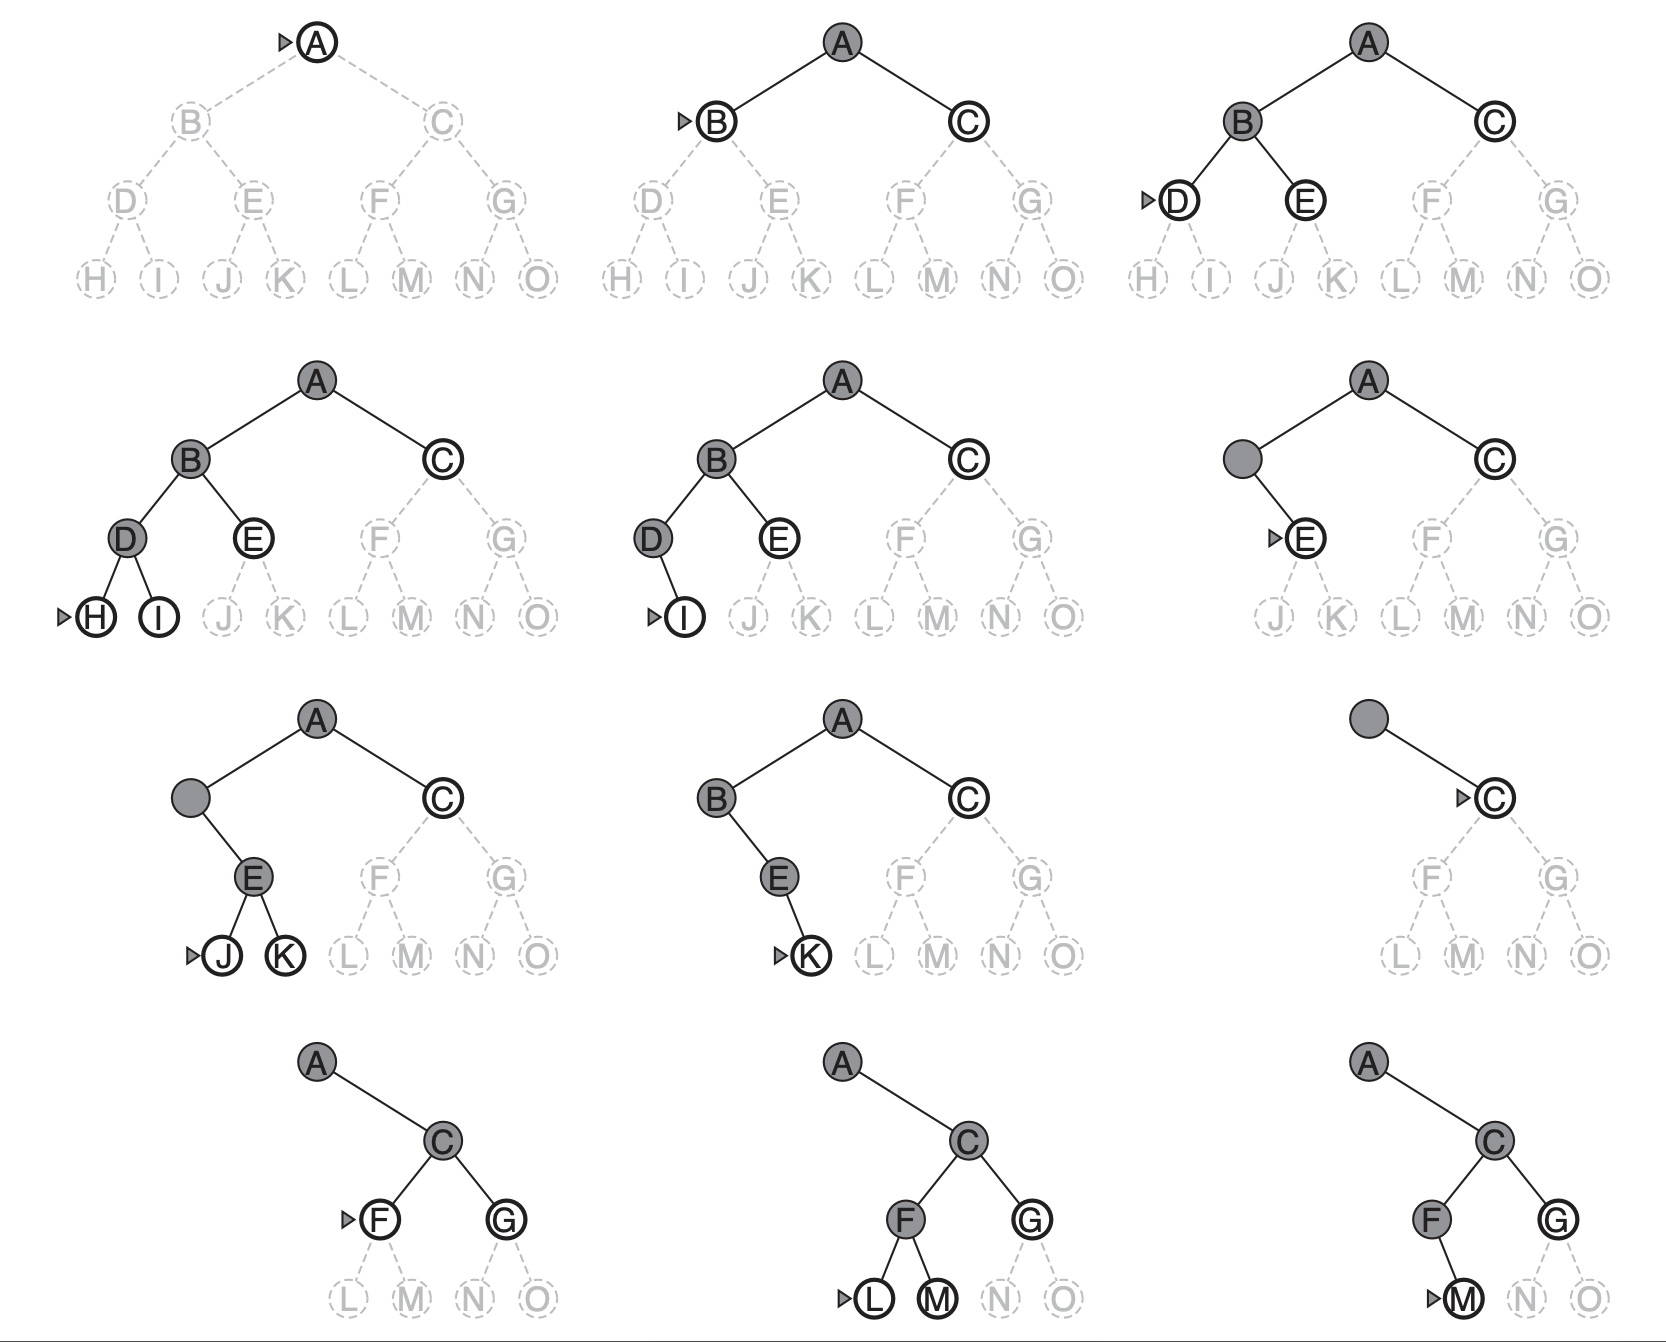
\includegraphics[width=1.0\textwidth]{images/tiefensuche.png}
	\caption{Tiefensuche in einem Binärbaum. $A$ ist der Startknoten und $M$ ist der Zielknoten, unentdeckte Knoten sind hellgrau. 
		Bereits entdeckte Knoten ohne weitere Unterknoten werden entfernt.}
	\label{fig:Tiefensuche}
\end{figure}

\section{Dijkstra Algorithmus}
\label{Dijkstra Algorithmus}

Der Dijkstra-Algorithmus (benannt nach seinem Entdecker E.W. Dijkstra) ist ein bekannter Algorithmus auf dem Gebiet der optimalen
Pfadwahl und wird verwendet, um den kürzesten Pfad von einem Startpunkt in einem Graphen zu einem Zielpunkt zu finden \cite{Javaid2019}.

\subsection{Funktionsprinzip}

Das Grundkonzept des Algorithmus ist wie folgt:
\\ \\
In einem ersten Schritt wird der Startknoten festgelegt und der Abstand zwischen ihm und den anderen Knoten des Graphen berechnet. 
Gibt es keine Kante, die diesen Knoten mit dem Startpunkt verbindet, ist der Abstand unendlich; gibt es eine Kante, die 
diesen Knoten mit dem Startpunkt verbindet, ist der Abstand $n$; und das niedrigste Gewicht (wenn es mehrere Kanten gibt) ist $n$.

Der zweite Schritt besteht darin, den Punkt mit dem kürzesten Abstand zum Startpunkt zu ermitteln und zu speichern. Die zuvor ermittelte 
Entfernung wird mit derjenigen verglichen, die über den soeben beiseite gelegten Scheitelpunkt für alle verbleibenden Scheitelpunkte 
ermittelt wurde, und nur der kleinste der beiden Werte wird beibehalten. Dieser Vorgang wird so lange wiederholt, bis es keine Scheitelpunkte
mehr gibt oder bis der Ankunftsscheitelpunkt gewählt ist \cite{Zhou:19}.

Der Dijkstra-Algorithmus arbeitet mit der Zuweisung einiger vorläufiger Entfernungswerte und versucht, diese schrittweise zu verbessern.
Der Pseudocode des Algorithmus ist in der Abbildung \ref{fig:Dijkstra Pseudo-Code}  dargestellt \cite{Huang2012}.
\\ \\
\\ \\
Im Folgenden wird die Umsetzung des unten stehenden Pseudocodes erläutert, angelehnt an \cite{Abusalim2020}.

Beim Dijkstra-Algorithmus ist die Route unbekannt. Die Knoten werden als temporär $(t)$ oder permanent $(p)$ eingestuft.
\begin{itemize}
	\item Schritt1: die Entfernung des Quellknotens wird der Wert Null zugewiesen $[distance (source) = 0]$, und die Entfernung der anderen
		Knoten wird auf unendlich gesetzt $[distance(x) = Infinity]$.
	\item Schritt 2: Suche des Knotens $x$ mit der kürzesten Entfernung $d(x)$. Wenn $d(x)$ unendlich ist oder es keine temporären Knoten gibt,
		wurde der Knoten $x$ als permanent markiert, was bedeutet, dass sich $d(x)$ und sein übergeordneter Wert nicht ändern werden.
	\item Schritt 3: Für jeden temporären Knoten mit dem Label $y$, der an $x$ angrenzt, wird der folgende Vergleich durchgeführt:

	
\end{itemize}
% \begin{gather*} \label{eq:2.1}
wenn
\begin{equation} \label{eq:2.1}
	d(x) + w (x, y) < d(y)	
\end{equation}
dann
\begin{equation} \label{eq:2.2}
	D(y) = d(x) + w (x, y)
\end{equation}
\newline
Wenn die Entfernung des gekennzeichneten Knotens $d(y)$ größer ist als die Entfernung des gekennzeichneten Knotens $d(x)$ plus Verbindungsgewicht $w(x, y)$, 
wird die Entfernung des gekennzeichneten Knotens $y$ gemäß den Gleichungen \ref{eq:2.1} und \ref{eq:2.2} aktualisiert in $D(y)$.

\noindent \\
\begin{minipage}{1.0\textwidth} \small
\begin{lstlisting}
$\textbf{function}$ DIJKSTRA (Graph, source)
	create vertex set D
	for each vertex v in Graph:
		distance[v] $\leftarrow$ INFINITY
		previous[v] $\leftarrow$ UNDEFINED
\end{lstlisting}
\captionof{lstlisting}{Dijkstra Algorithmus Pseudocode}
\end{minipage}

% PSEUDOCODE BILD - LÖSCHEN
\begin{figure}[H]
	\centering
	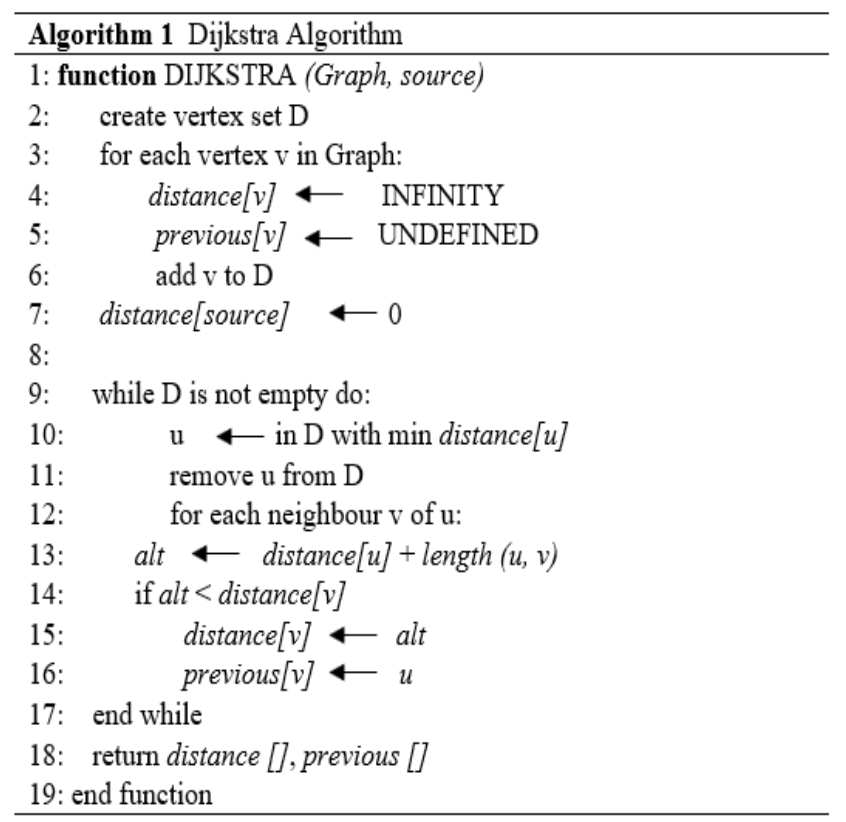
\includegraphics[width=1.0\textwidth]{images/Dijkstra_pseudoCode.PNG}
	\caption{Dijkstra Algorithmus Pseudo-Code, angelehnt an \cite{Abusalim2020}.}
	\label{fig:Dijkstra Pseudo-Code}
\end{figure}

\subsection{Vor- und Nachteile}
Der Dijkstra-Algorithmus hat zwei wesentliche Vorteile: Er kann alle optimalen Pfade finden und die Trefferquote dafür liegt
bei 100\%. Der zweite Vorteil ist, dass er die verbleibenden unerwünschten Knoten nicht besucht, wenn der beabsichtigte Zielknoten erreicht
ist \cite{Zhou:19,Abusalim2020}.
\\ \\
Der Hauptnachteil des Algorithmus besteht darin, dass er eine blinde Suche durchführt, was eine erhebliche Menge an Zeit und Ressourcen vergeudet. 
Ein weiterer Nachteil ist, dass er nicht mit negativen Kanten umgehen kann, was zu azyklischen Graphen führt, und daher nicht immer den kürzesten 
Weg findet \cite{Mukhlif:20}.


\section{Bellman-Ford Algorithmus}
\label{Bellman-Ford-Algorithmus}

In 1958 veröffentlichte Richard Bellman den Bellman-Ford-Algorithmus, einen Graphen-Suchalgorithmus zur Ermittlung des kürzesten 
Pfades \cite{Abusalim2020,Sulaiman18}.
\subsection{Eigenschaften}
Um kürzeste Wege auf gerichteten Graphen zu finden, nutzt der Bellman-Ford-Algorithmus die Relaxation.
Relaxation bedeutet, dass geprüft wird, ob es möglich ist, den Weg zu dem Knoten, auf den die Kante zeigt, zu verkürzen, 
und wenn dies der Fall ist, wird der Weg zum Knoten durch den entdeckten Weg ersetzt.
Der Bellman-Ford Algorithmus kann auch mit negative Kantengewichten umgehen. 
Wenn es Zyklen mit negativem Gewicht gibt, wird der Algorithmus sie erkennen (so dass es keine Lösung gibt) \cite{Vaibhavi2014}.

Die Vorteile dieses Algorithmus sind unter anderem, dass es sich um einen dynamischen Algorithmus handelt, dass er negative gerichtete 
Kanten (und auch positive) berechnen kann, dass er die Kosten für den Aufbau des Netzes reduzieren kann, indem er den kürzesten Weg von einem 
Knoten zum anderen findet, und dass er die Anzahl der aufgebauten Router-Pfad reduzieren kann \cite{Abusalim2020}.

\subsection{Funktionsprinzip}\index{Bellman-Ford}

Angelehnt an \cite{Abusalim2020} wird der Bellman-Ford-Algorithmus wie folgt ausgeführt:
\\
\begin{itemize}
	\item Schritt 1: Zuweisung des Abstandswertes des Startpunktes $s$ zu null $(distance[s] = 0)$ und des Abstandswertes der anderen Punkte zu 
		$INFINITY$.
	\item Schritt 2: Wenn $n$ die Anzahl der Knoten ist, wird jede Kante $(n - 1)$ Mal relaxiert. 
	\item Schritt 3: Mit der N-ten Schleife wird geprüft, ob der Graph negative Zyklen aufweist.
\end{itemize}
Der Bellman-Ford-Algorithmus wird wie in Listing 2.2 unten dargestellt ausgeführt.

\noindent \\
\begin{minipage}{1.0\textwidth} \small
\begin{lstlisting}[label=lst:Bellman-Ford]
$\textbf{function}$ bellmanFord (G, s)
	for each vertex V in G:
		distance[v] $\leftarrow$ INFINITY
		previous[v] $\leftarrow$ NULL
		
\end{lstlisting}
\captionof{lstlisting}{Bellman-Ford-Algorithmus Pseudocode}
\end{minipage}


% PSEUDOCODE BILD - LÖSCHEN
\begin{figure}[H]
	\centering
	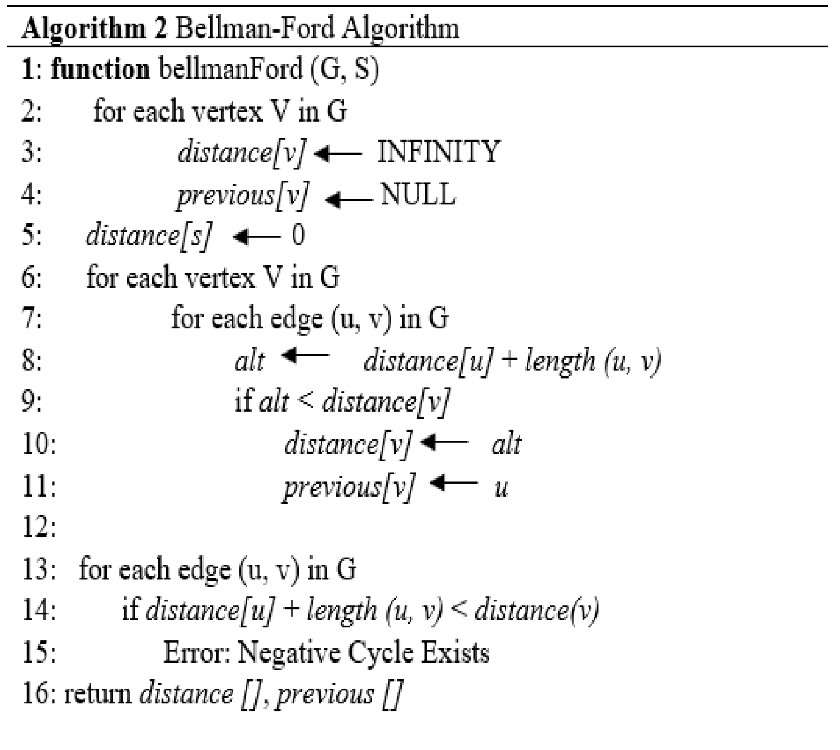
\includegraphics[width=1.0\textwidth]{images/Bellman-Ford-Algorithmus_Pseudo-Code.PNG}
	\caption{Bellman-Ford Pseudo-Code, angelehnt an\cite{Abusalim2020}.}
	\label{fig:Bellman-Ford Pseudo-code}
\end{figure}






